
\section{\trMorse\trTrajectory{}与\trFloer\trTrajectory{}的一致}
\label{sec:trajectories-coincide}

\subsection{与 $t$ 无关的\trTrajectory{}是\trRegular{}的}
\label{subsec:t-independent-regular}

我们现在来证明\cref{thm:kernel-df-equals-lu}（以及\cref{thm:df-surjective-along-gradient}）。显然有 $\operatorname{Ker}L_{u}\subset\operatorname{Ker}(d\scr{F})_{u}$：如果 $Y(s)$ 满足
\[
\frac{dY}{ds}+S(s)Y=0\text{，}
\]
那么它也满足
\[
\frac{\partial Y}{\partial s}+J\frac{\partial Y}{\partial t}+S(s)Y=0\text{。}
\]
让我们来证明相反的包含关系。我们令 $L=(d\scr{F})_{u}$ 与 $L_{0}=L_{u}$。设 $Y\in\operatorname{Ker}L$。我们有
\[
\int_{0}^{1}J\frac{\partial Y}{\partial t}\,dt=0\text{，}\qquad\text{从而 }\ \int_{0}^{1}Y(s,t)\,dt\in\operatorname{Ker}L_{0}\text{。}
\]
于是我们可以——而且我们也确实如此——假定 $\int_{0}^{1}Y(s,t)\,dt=0$。我们要利用一条关于实变量函数的初等引理（它的证明稍后给出）。

\begin{lemma}\label{thm:mean-zero-inequality}
设 $f$ 是 $[0,1]$ 上的一个可微映射，它在这个区间上的平均值为零。那么对每个 $p\ge1$，我们有
\[
\int_{0}^{1}\|f(t)\|^{p}\,dt\le\int_{0}^{1}\|f'(t)\|^{p}\,dt\text{。}
\]
\end{lemma}

我们把它应用于 $f(t)=Y(s,t)$ 与 $p=2$，随后对 $s$ 积分：
\[
\int_{-\infty}^{+\infty}\int_{0}^{1}\bigl\|Y(s,t)\bigr\|^{2}\,dt\,ds
\le\int_{-\infty}^{+\infty}\int_{0}^{1}\Bigl\|\frac{\partial Y}{\partial t}(s,t)\Bigr\|^{2}\,dt\,ds\text{。}
\]
对于 $L^{2}$ 范数，我们有
\[
\begin{aligned}
\Bigl\|\frac{\partial Y}{\partial s}\Bigr\|^{2}_{L^{2}}+\Bigl\|\frac{\partial Y}{\partial t}\Bigr\|^{2}_{L^{2}}
&=\Bigl\langle\frac{\partial Y}{\partial s},\,\frac{\partial Y}{\partial s}\Bigr\rangle+\Bigl\langle\frac{\partial Y}{\partial t},\,\frac{\partial Y}{\partial t}\Bigr\rangle\\
&=-\langle Y,\,\Delta Y\rangle\\
&=-\Bigl\langle Y,\,\Bigl(\frac{\partial}{\partial s}-J\frac{\partial}{\partial t}\Bigr)\Bigl(\frac{\partial}{\partial s}+J\frac{\partial}{\partial t}\Bigr)Y\Bigr\rangle\\
&=\Bigl\|\frac{\partial Y}{\partial s}+J\frac{\partial Y}{\partial t}\Bigr\|^{2}_{L^{2}}\\
&=\|S(s)Y\|^{2}_{L^{2}}\\
&\le\sup_{s}\|S(s)\|^{2}\,\|Y\|^{2}_{L^{2}}
\end{aligned}
\]
（利用了 $S(s)$ 的算子范数）。于是，由我们的这条引理，我们得到
\[
\|Y\|^{2}_{L^{2}}\le\|\operatorname{grad}Y\|^{2}_{L^{2}}\le\sup_{s}\|S(s)\|^{2}\,\|Y\|^{2}_{L^{2}}\text{。}
\]
$H$ 是“$\cC^{2}$-小”的这一事实蕴含 $\sup_{s}\|S(s)\|$ 充分小，从而 $Y=0$。\noqed

\begin{proof}[\cref{thm:mean-zero-inequality}的证明]
设 $t$、$t_{1}\in[0,1]$，我们写
\[
f(t_{1})-f(t)=\int_{t}^{t_{1}}f'(\tau)\,d\tau\text{。}
\]
随后我们把这个关系式关于 $t$ 在 $0$ 与 $1$ 之间积分，得
\[
f(t_{1})=\int_{0}^{1}\Bigl(\int_{t}^{t_{1}}f'(\tau)\,d\tau\Bigr)dt\text{，}
\]
由此我们推出\footnote{译注：原书此链当 $t_{1}<t$ 时有漏洞：此时 $\int_{t}^{t_{1}}$ 是反向积分，以这种积分限写出的估计 $\bigl\|\int_{t}^{t_{1}}f'(\tau)\,d\tau\bigr\|^{p}\le\int_{t}^{t_{1}}\|f'(\tau)\|^{p}\,d\tau$ 不能成立（右端非正而左端非负）。修补办法是把积分限换成 $\int_{\min(t,t_{1})}^{\max(t,t_{1})}$：一方面，由区间长不超过 $1$ 与\trHoelder{}不等式，$\bigl\|\int_{t}^{t_{1}}f'(\tau)\,d\tau\bigr\|^{p}\le\int_{\min(t,t_{1})}^{\max(t,t_{1})}\|f'(\tau)\|^{p}\,d\tau$ 仍然成立；另一方面，由 Fubini 定理，$\int_{0}^{1}\!\int_{0}^{1}\int_{\min(t,t_{1})}^{\max(t,t_{1})}g(\tau)\,d\tau\,dt\,dt_{1}=\int_{0}^{1}2\tau(1-\tau)g(\tau)\,d\tau\le\int_{0}^{1}g(\tau)\,d\tau$，故最末一步不等式依旧成立（亦可径以全区间上 $\|f'\|_{L^{p}}$ 的界控制之）。此处照原书排印，载此更正。——译者注}
\[
\int_{0}^{1}\bigl\|f(t_{1})\bigr\|^{p}\,dt_{1}
\le\int_{0}^{1}\Bigl(\int_{0}^{1}\int_{t}^{t_{1}}\|f'(\tau)\|^{p}\,d\tau\,dt\Bigr)dt_{1}
\le\int_{0}^{1}\|f'(\tau)\|^{p}\,d\tau\text{，}
\]
这正是所要证明的。
\end{proof}

\subsection{\trTrajectory{}与 $t$ 无关}
\label{subsec:trajectories-independent-t}

我们现在来证明：$H/k$ 的那些被计入\trFloerComplex{}的\trTrajectory，恰好就是那些被计入\trMorseComplex{}的\trTrajectory；换句话说，也就是\cref{thm:hk-large-t-independent}。

\begin{proof}[\cref{thm:hk-large-t-independent}的证明]
我们假定它不成立。这意味着：存在一个趋于无穷的序列 $(n_{k})$，以及\trFloerEquation
\[
\frac{\partial u}{\partial s}+J\frac{\partial u}{\partial t}+\frac{1}{n_{k}}\operatorname{grad}H=0
\]
的一个解 $u_{n_{k}}$（它确实依赖于 $t$），我们可以假定它把\trCriticalPoint{} $x$ 与 $y$ 连接起来。令
\[
v_{n_{k}}(s,t)=u_{n_{k}}(n_{k}s,n_{k}t)\text{。}
\]
这是原先那个\trHamiltonian{}量 $H$ 的\trFloerEquation{}的一个解，它以 $1/n_{k}$ 为\trPeriodic；从而我们可以把它视为以 $1$ 为\trPeriodic，于是 $v_{n_{k}}\in\scr{M}(x,y,H)$。

先考虑\trIndex{}之差为 $1$ 的情形，
\[
\operatorname{Ind}(x)-\operatorname{Ind}(y)=1=\mu(x)-\mu(y)\text{。}
\]
由朝\trBrokenTrajectory{}的\trConvergence{}定理（\cref{thm:broken-limit-decomposition}），在必要时抽取一个子序列之后，我们可以——而且我们也确实如此——假定序列 $(v_{n_{k}})$ 趋于一个极限 $v\in\scr{M}(x,y,H)$。如果我们证明了 $v$ 不依赖于 $t$，那么由于 $(d\scr{F})_{v}$ 是\trSurjective{}的（按\cref{thm:df-surjective-along-gradient}），$v$ 就必定落在 $\scr{M}(x,y,H)$ 的一个维数为 $1$ 的\trConnectedComponent{}之中，也就是说，必定是 $\scr{L}(x,y)$ 的一个\trIsolated{}点。于是，对充分大的 $k$，我们就会有
\[
v_{n_{k}}(s,t)=v(s+\sigma_{k},t)=v(s+\sigma_{k})\text{，}
\]
从而 $v_{n_{k}}$ 就不依赖于 $t$ 了，这与我们所做的假设相矛盾。

因此，只需证明极限 $v$ 不依赖于 $t$。我们要利用这样一个事实：$v$ 是一个\trPeriodic{}趋于 $0$ 的序列的极限。设 $r\in\RR$。我们取定一个 $s\in\RR$ 与一个 $t\in[0,1]$。由于 $v_{n_{k}}$ 以 $1/n_{k}$ 为\trPeriodic，我们有
\[
v_{n_{k}}(s,t)=v_{n_{k}}\Bigl(s,\ t+\frac{[rn_{k}]}{n_{k}}\Bigr)
\]
（其中 $[rn_{k}]$ 表示 $rn_{k}$ 的整数部分）。当 $k$ 趋于无穷时，$[rn_{k}]/n_{k}$ 趋于 $r$，于是左边趋于 $v(s,t)$，而右边趋于 $v(s,t+r)$。从而，对每个 $r$，
\[
v(s,t)=v(s,t+r)\text{，}
\]
这正是所要证明的。

现在我们假定\trIndex{}之差为 $2$，
\[
\operatorname{Ind}(x)-\operatorname{Ind}(y)=2=\mu(x)-\mu(y)\text{。}
\]
在这种情形下，\cref{thm:broken-limit-decomposition}断言：$(v_{n_{k}}(s+s_{k},t))$ 的一个子序列要么趋于一个极限 $v\in\scr{M}(x,y,H)$，要么趋于一条\trBrokenTrajectory
\[
(v,w)\in\scr{M}(x,z)\times\scr{M}(z,y)\text{。}
\]
在第一种情形，我们如同上面那样证明 $v$ 与 $t$ 无关。再一次，$(d\scr{F})_{v}$ 按\cref{thm:df-surjective-along-gradient}是\trSurjective{}的。于是，正如\cref{thm:regular-values-pi}的证明中那样，我们发现在 $(v,H)$ 的一个邻域内，$\scr{M}(x,y,H)$ 是 $\scr{Z}(x,y,J)$ 的一个维数为 $2$ 的\trSubmanifold（我们利用第~8~章中的记号
\[
\scr{Z}(x,y,J)=\bigl\{(v,H+h)\ \bigm|\ h\in\cC^{\infty}_{\varepsilon}(H),\ v\in\scr{M}(x,y,J,H+h)\bigr\}
\]
）。此外，由于 $H$ 的\trGradient{} $-JX_{H}$ 具有\trSmale{}性质，把 $x$ 连接到 $y$ 的那些\trTrajectory{}构成一个维数为 $2$ 的\trManifold。但是这些\trTrajectory{}也在 $\scr{M}(x,y,H)$ 之中，从而我们便在 $v$ 的邻域内得到了这个\trSubmanifold{}的一个由不依赖于 $t$ 的\trTrajectory{}所给出的\trParametrization。其次，由于 $v_{n_{k}}(s+s_{k},t)\in\scr{M}(x,y,H)$，并且这个序列趋于 $v$，故对充分大的 $k$，$v_{n_{k}}(s+s_{k},t)$ 与 $t$ 无关，这是一个矛盾。

只剩下 $\lim v_{n_{k}}=(v,w)$ 的情形了，也就是说：存在序列 $(s_{k}^{1})$ 与 $(s_{k}^{2})$，使得
\[
\lim_{k\to+\infty}v_{n_{k}}(s+s_{k}^{1},t)=v(s,t)
\qquad\text{与}\qquad
\lim_{k\to+\infty}v_{n_{k}}(s+s_{k}^{2},t)=w(s,t)\text{。}
\]
如同上面那样，我们证明 $v$ 与 $w$ 不依赖于 $t$。按\cref{thm:df-surjective-along-gradient}，两个算子 $(d\scr{F})_{v}$ 与 $(d\scr{F})_{w}$ 都是\trSurjective{}的。于是我们可以应用\trGluing{}定理（\cref{thm:gluing-psi}）。由此我们推出：存在一个\trEmbedding
\[
\widehat{\psi}\colon[\rho_{0},+\infty[\ \longrightarrow\scr{L}(x,y)
\]
使得
\[
\lim_{\rho\to+\infty}\widehat{\psi}(\rho)=(\widehat{v},\widehat{w})\in\scr{L}(x,z)\times\scr{L}(z,y)\text{。}
\]
另一方面，$v$ 与 $w$ 也是\trSmale\trVectorField{} $-JX_{H}$ 的（\trMorse{}）\trTrajectory。在这个框架下，\trGluing{}定理（即\cref{thm:broken-manifold-boundary}）断言：\footnote{译注：原书此处印作 $(\widehat{u},\widehat{v})$；按上下文，此处的极限偶对为 $(\widehat{v},\widehat{w})$（见前注），疑为排印之误。此处照原书排印，存疑备案。——译者注}\trBrokenTrajectory{} $(\widehat{u},\widehat{v})$ 是一个由把 $x$ 连接到 $y$ 的\trMorse{}\trTrajectory{}所组成的、维数为 $1$ 的\trManifold{}的边界点。但是这些\trTrajectory{}同时也是\trFloer{}\trTrajectory，于是我们有一条映射
\[
\varphi\colon[\rho_{0},+\infty[\ \longrightarrow\scr{M}(x,y,H)
\]
使得
\[
\widehat{\varphi}\colon[\rho_{0},+\infty[\ \longrightarrow\scr{L}(x,y)
\]
是一个\trEmbedding。此外，当 $\rho$ 趋于 $+\infty$ 时，$\widehat{\varphi}(\rho)$ 便在\trMorse{}理论中朝\trBrokenTrajectory{}的\trConvergence{}的意义（该意义定义于\cref{subsec:space-broken-trajectories}中）下趋于 $(\widehat{v},\widehat{w})$。特别地，这意味着
\[
\lim_{\rho\to+\infty}\varphi(\rho)\bigl(s_{\rho}^{+}\bigr)=v\bigl(s^{+}\bigr)\text{，}
\]
其中 $s_{\rho^{+}}$ 与 $s^{+}$ 分别表示\trTrajectory{} $\varphi(\rho)$ 与 $v$ 在 $x$ 的一个（取定的）\trMorse{}邻域处的\trExitPoint。这就蕴含：对于 $\cC^{\infty}_{\mathrm{loc}}$ \trTopology，
\[
\lim_{\rho\to+\infty}\varphi(\rho)\bigl(s+s_{\rho}^{+}\bigr)=v\bigl(s+s^{+}\bigr)
\]
（要看出这一点，只需写出
\[
\varphi(\rho)\bigl(s+s_{\rho}^{+}\bigr)=\Phi_{s}\bigl(\varphi(\rho)(s_{\rho}^{+})\bigr)
\qquad\text{与}\qquad
v\bigl(s+s^{+}\bigr)=\Phi_{s}\bigl(v(s^{+})\bigr)\text{，}
\]
其中 $\Phi_{s}$ 是 $-JX_{H}$ 的\trFlow）。

同样的推理也适用于 $w$。于是我们便得到了：在\trFloer{}理论中朝\trBrokenTrajectory{}的\trConvergence{}的意义（该意义由\cref{thm:broken-limit-decomposition}定义）下，
\[
\lim_{\rho\to+\infty}\widehat{\varphi}(\rho)=(\widehat{v},\widehat{w})\text{。}
\]

总而言之，我们有三重趋于 $(\widehat{v},\widehat{w})$ 的\trConvergence{}（\cref{fig:three-convergences}）：
\begin{itemize}
\item 我们所假设的、$(v_{n_{k}})$ 当 $k$ 趋于无穷时的\trConvergence；
\item 由“\trFloer{}”\trGluing{}所给出的、$\widehat{\psi}(\rho)$ 当 $\rho\to+\infty$ 时的\trConvergence；
\item 由“\trMorse{}”\trGluing{}所给出的、$\widehat{\varphi}(\rho)$ 当 $\rho\to+\infty$ 时的\trConvergence。
\end{itemize}

\begin{figure}[htbp]
\centering
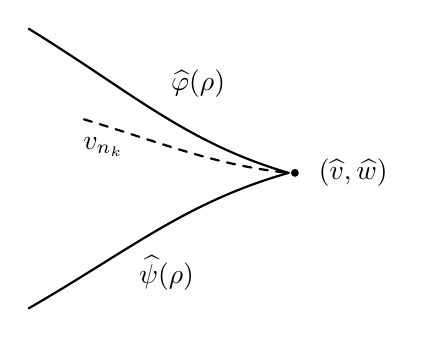
\begin{tikzpicture}[line cap=round,line join=round]
\draw[thick] (-2.7,1.95) .. controls (-1.4,1.15) and (-0.7,0.5) .. (0.6,0.12);
\node at (-0.55,1.25) {$\widehat{\varphi}(\rho)$};
\draw[dashed,thick] (-2.0,0.8) .. controls (-1.0,0.5) and (-0.35,0.22) .. (0.6,0.12);
\node at (-1.75,0.45) {$v_{n_{k}}$};
\draw[thick] (-2.7,-1.6) .. controls (-1.4,-0.85) and (-0.7,-0.25) .. (0.6,0.12);
\node at (-0.95,-1.15) {$\widehat{\psi}(\rho)$};
\fill (0.68,0.12) circle (0.05);
\node at (1.42,0.12) {$(\widehat{v},\widehat{w})$};
\end{tikzpicture}
\caption{}
\label{fig:three-convergences}
\end{figure}

现在我们应用\trGluing{}定理（\cref{thm:gluing-psi}）的“唯一性”部分。它蕴含：对充分大的 $k$，$(v_{n_{k}})$ 落在 $\widehat{\psi}$ 的像之中。同样的唯一性论证还蕴含：对充分大的 $\rho$，比方说 $\rho\ge\rho_{1}$，$\widehat{\varphi}(\rho)\in\operatorname{Im}\widehat{\psi}$。此外，$\widehat{\varphi}([\rho_{1},+\infty[)$ 是维数为 $1$ 的\trManifold{} $\scr{L}(x,y)$ 中的一个区间。由于
\[
\lim_{\rho\to+\infty}\widehat{\varphi}(\rho)=\lim_{\rho\to+\infty}\widehat{\psi}(\rho)=(\widehat{v},\widehat{w})\notin\scr{L}(x,y)\text{，}
\]
这就意味着：对充分大的 $\rho$，$\widehat{\psi}(\rho)\in\operatorname{Im}\widehat{\varphi}$。特别地，对充分大的 $k$，$\widehat{v}_{n_{k}}\in\operatorname{Im}\widehat{\varphi}$，这与 $v_{n_{k}}$ 依赖于 $t$ 的事实相矛盾。\footnote{译注：原书此处印作 “which contradicts the fact that $v_{n_{k}}$ does not depend on $t$”；按本证明开篇的归谬设定（$u_{n_{k}}$ 确实依赖于 $t$，从而 $v_{n_{k}}$ 亦然），矛盾应针对“$v_{n_{k}}$ 依赖于 $t$”，原书多一枚 not，此处径改删去。——译者注}
\end{proof}

我们现已证明：把两个相邻\trCriticalPoint{}连接起来的所有\trFloer{}解都是\trMorse{}\trTrajectory，并且 $(d\scr{F})_{v}$ 沿这些\trTrajectory{}是\trSurjective{}的。于是我们便有了诸\trComplex{}之间所期望的那个等式。
